\documentclass[a4paper,12pt]{article}
\usepackage[utf8]{inputenc}

\usepackage[top=2cm,bottom=2cm,right=1.5cm,left=1.5cm]{geometry}
\usepackage{amsmath,amssymb,enumitem,multicol,graphicx,tikz,framed,tcolorbox,mathtools,comment,subcaption,array,pgfplots}
\usepackage{listings}
\usepackage{xcolor}
\linespread{1.3}
%New colors defined below
\definecolor{codegreen}{rgb}{0,0.6,0}
\definecolor{codegray}{rgb}{0.5,0.5,0.5}
\definecolor{codepurple}{rgb}{0.58,0,0.82}
\definecolor{backcolour}{rgb}{0.95,0.95,0.92}
\definecolor{backcolour_two}{rgb}{1,1,1}

%Code listing style named "mystyle"
\lstdefinestyle{mystyle}{
  backgroundcolor=\color{backcolour},   commentstyle=\color{codegreen},
  keywordstyle=\color{magenta},
  numberstyle=\tiny\color{codegray},
  stringstyle=\color{codepurple},
  basicstyle=\ttfamily\footnotesize,
  breakatwhitespace=false,         
  breaklines=true,                 
  captionpos=b,                    
  keepspaces=true,                 
  numbers=left,                    
  numbersep=5pt,                  
  showspaces=false,                
  showstringspaces=false,
  showtabs=false,                  
  tabsize=2
}

\lstdefinestyle{mystyle_big}{
	backgroundcolor=\color{backcolour_two},   commentstyle=\color{codegreen},
	keywordstyle=\color{magenta},
	numberstyle=\tiny\color{codegray},
	stringstyle=\color{codepurple},
	basicstyle=\ttfamily\normalsize,
	breakatwhitespace=false,         
	breaklines=true,                 
	captionpos=b,                    
	keepspaces=true,                 
	numbers=left,                    
	numbersep=5pt,                  
	showspaces=false,                
	showstringspaces=false,
	showtabs=false,                  
	tabsize=2
}

%"mystyle" code listing set
\lstset{style=mystyle}

\title{Code Listing}
\date{ }
\begin{document}
\section{Introduction}
\lstinputlisting[language=Python, caption=Python example
]{first_class.py}

\begin{figure} [!h]
	\centering
	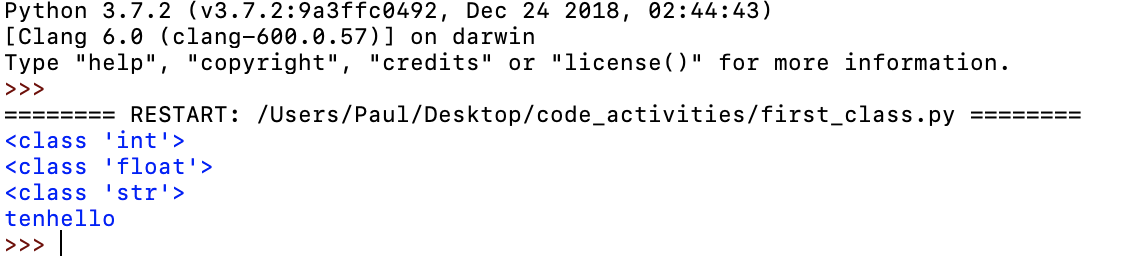
\includegraphics[width=18cm]{screen_shots/first_class.png}
	\caption*{Output}
\end{figure}
\newpage
\section{Basic Program}
\subsection{Dinner Order}
You need to create a program that allows a waiter to enter in the number of main meals ( at \$12.50 each ) , the number of desserts ( at \$6.00 each ) and the number of drinks ( at \$3.55 ) ordered at a table.\\
The program then prints out a summary of the order, a total and then adds on GST (and gives the new total ).\\
(Note: the program should be easy to alter so the price values should be declared as constant variables)


\begin{figure} [!h]
	\centering
	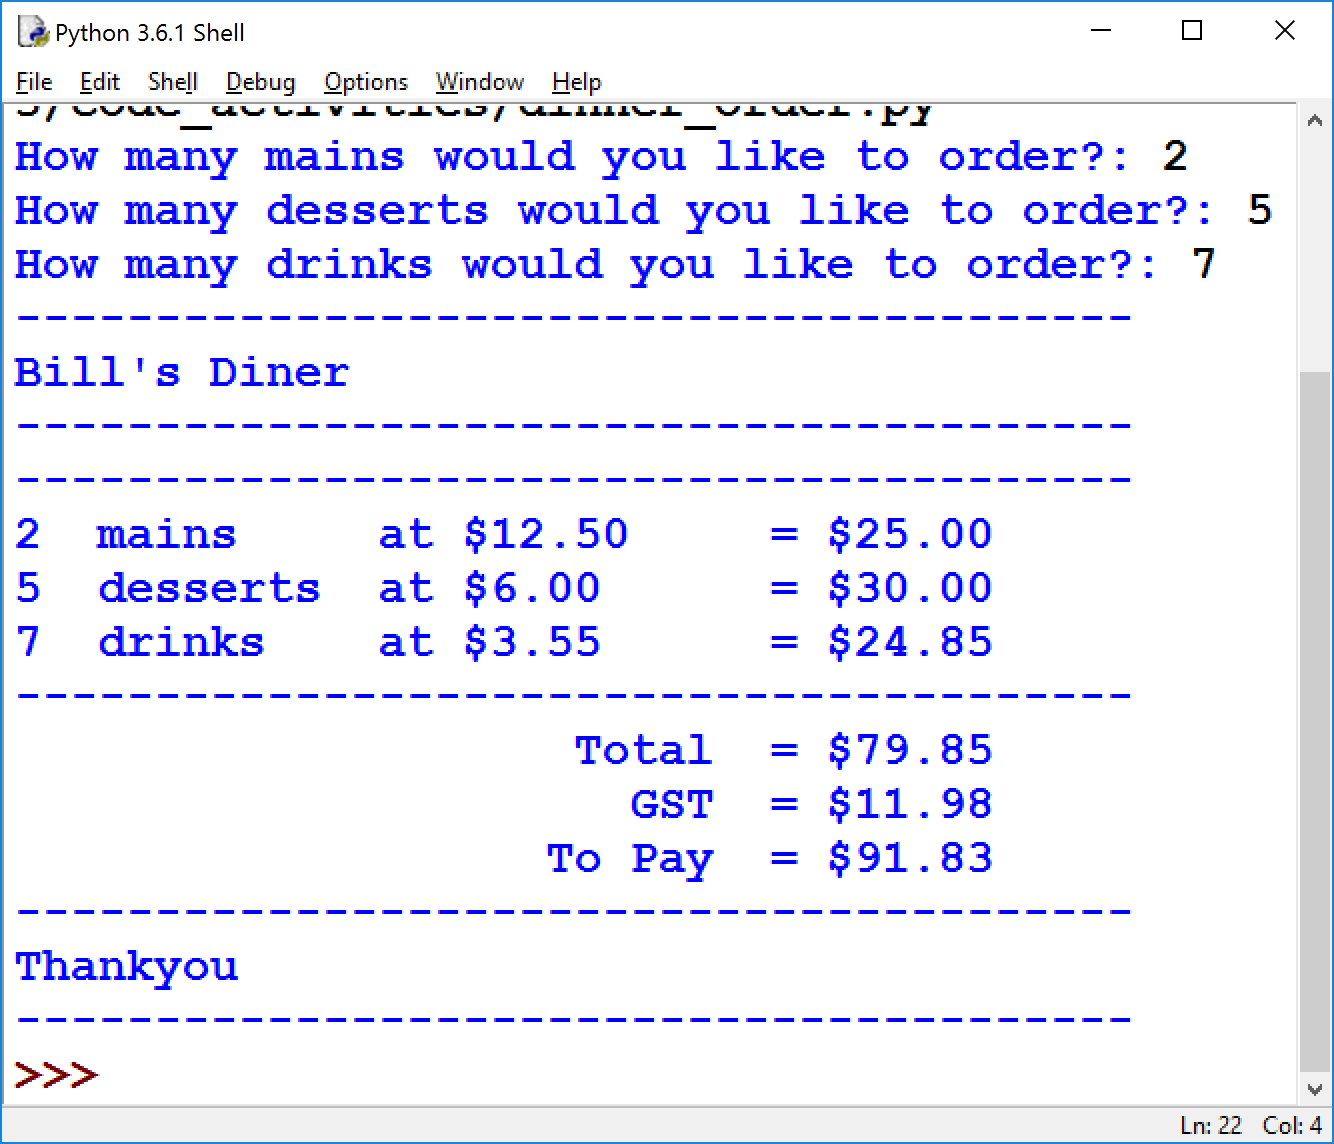
\includegraphics[width=10cm]{screen_shots/diner.png}
	\caption*{An example of Dinner Order program run}
\end{figure}


\subsubsection{Planning}
For the writing and planning:
\begin{itemize}
	\item \textbf{Decomposition}
Please write down your task decomposition.\\
(This is breaking the task down into smaller pieces that will be combined to make the finished program)\\
See examples below.
\item \textbf{Version Log}\\
Your version log should go here.  Annotated screenshots are a good idea at this point
\item \textbf{Component Trialling}\\
Show that you have trialled each component here.  \\
You should also include notes that justify the major decisions you made.
\item \textbf{Assembled Outcome Testing}\\
Please show testing for your assembled outcome below. \\
This should include a test plan followed by screenshot proof
\item \textbf{Usability Testing}\\
Try the program out on someone else and make notes or video etc.
Write a list of things improvements which need to be made based on your usability testing.  Then write down what you changed.
\item \textbf{General Evaluation:}\\
How good is may program? What can I do to improve it?
\end{itemize}


\textbf{Examples of Component Planning}\\
\begin{figure} [!h]
	\centering
	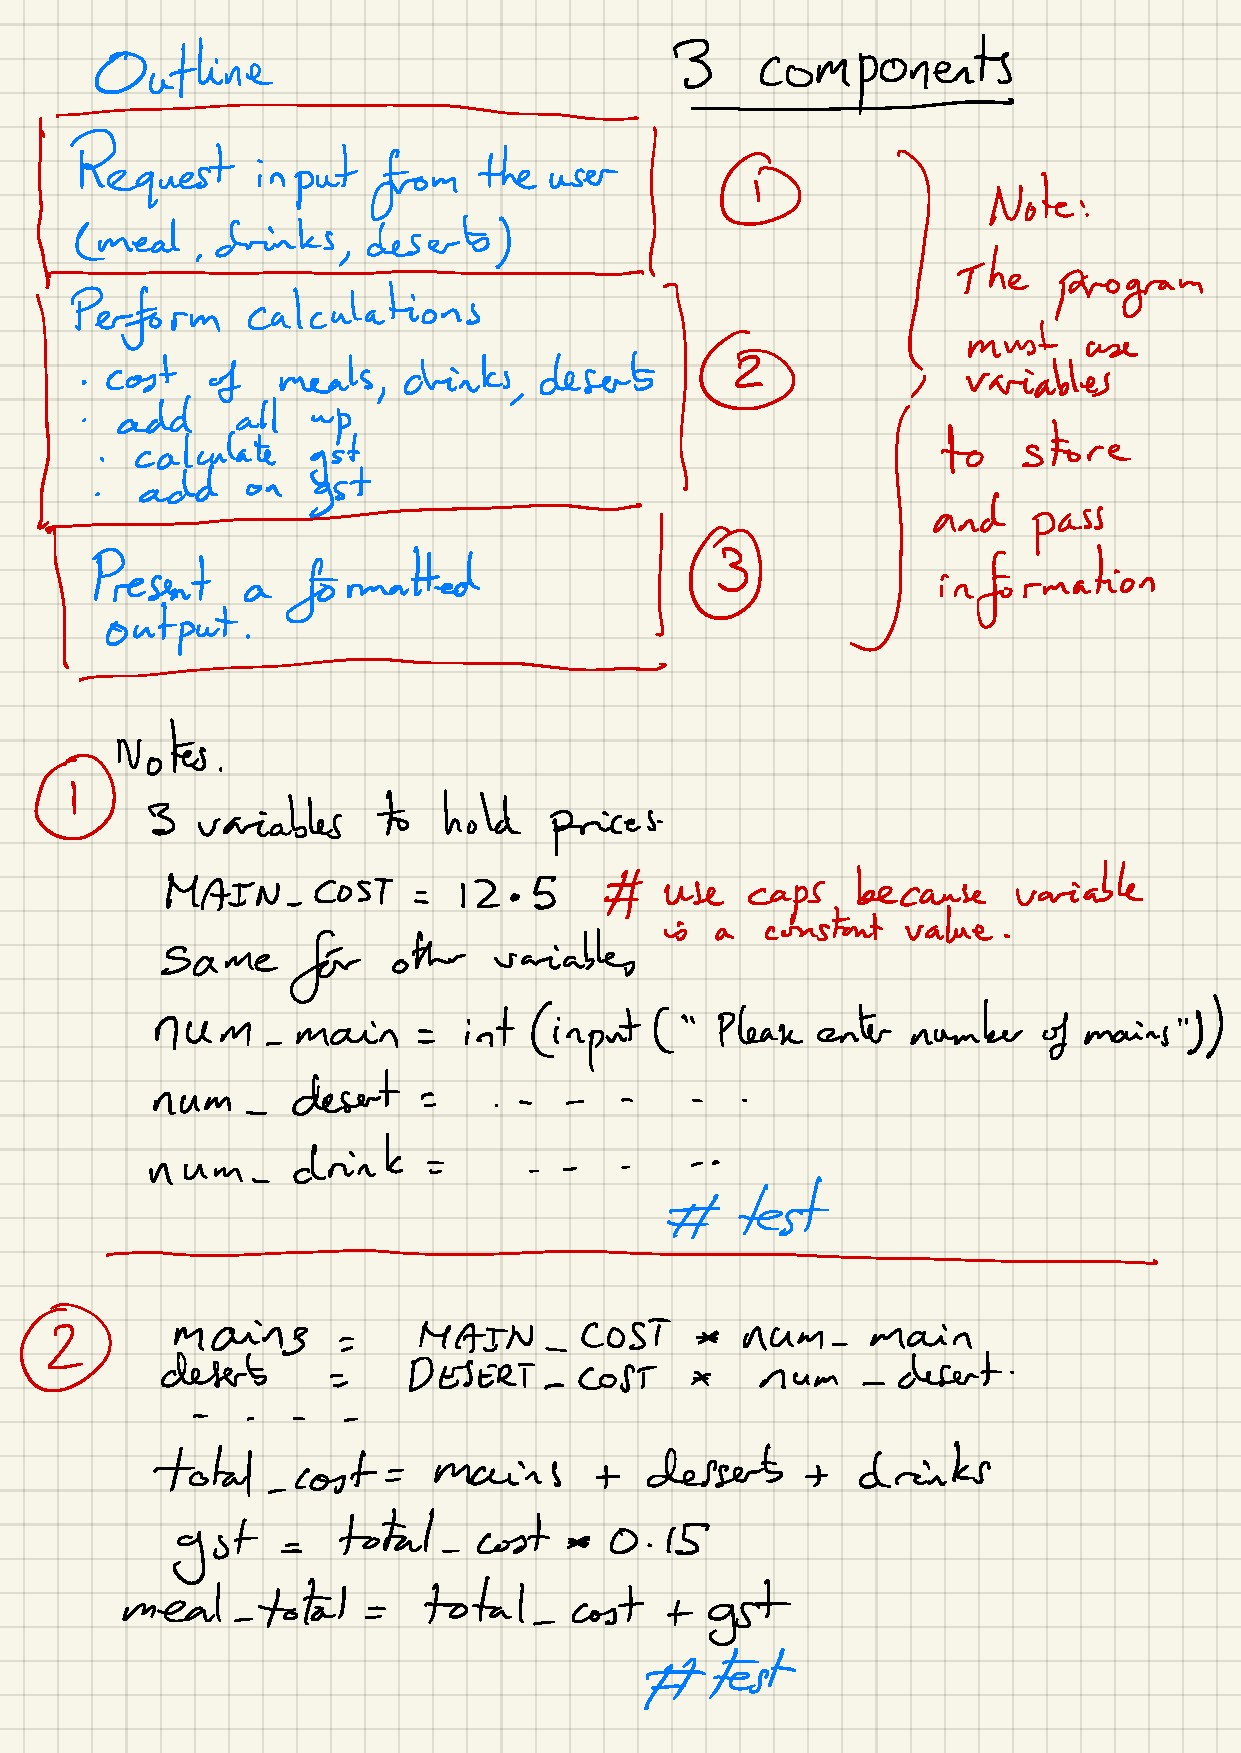
\includegraphics[width=12cm]{iterative_processes/simple_planning_1.pdf}
\end{figure}
\begin{figure} [!h]
	\centering
	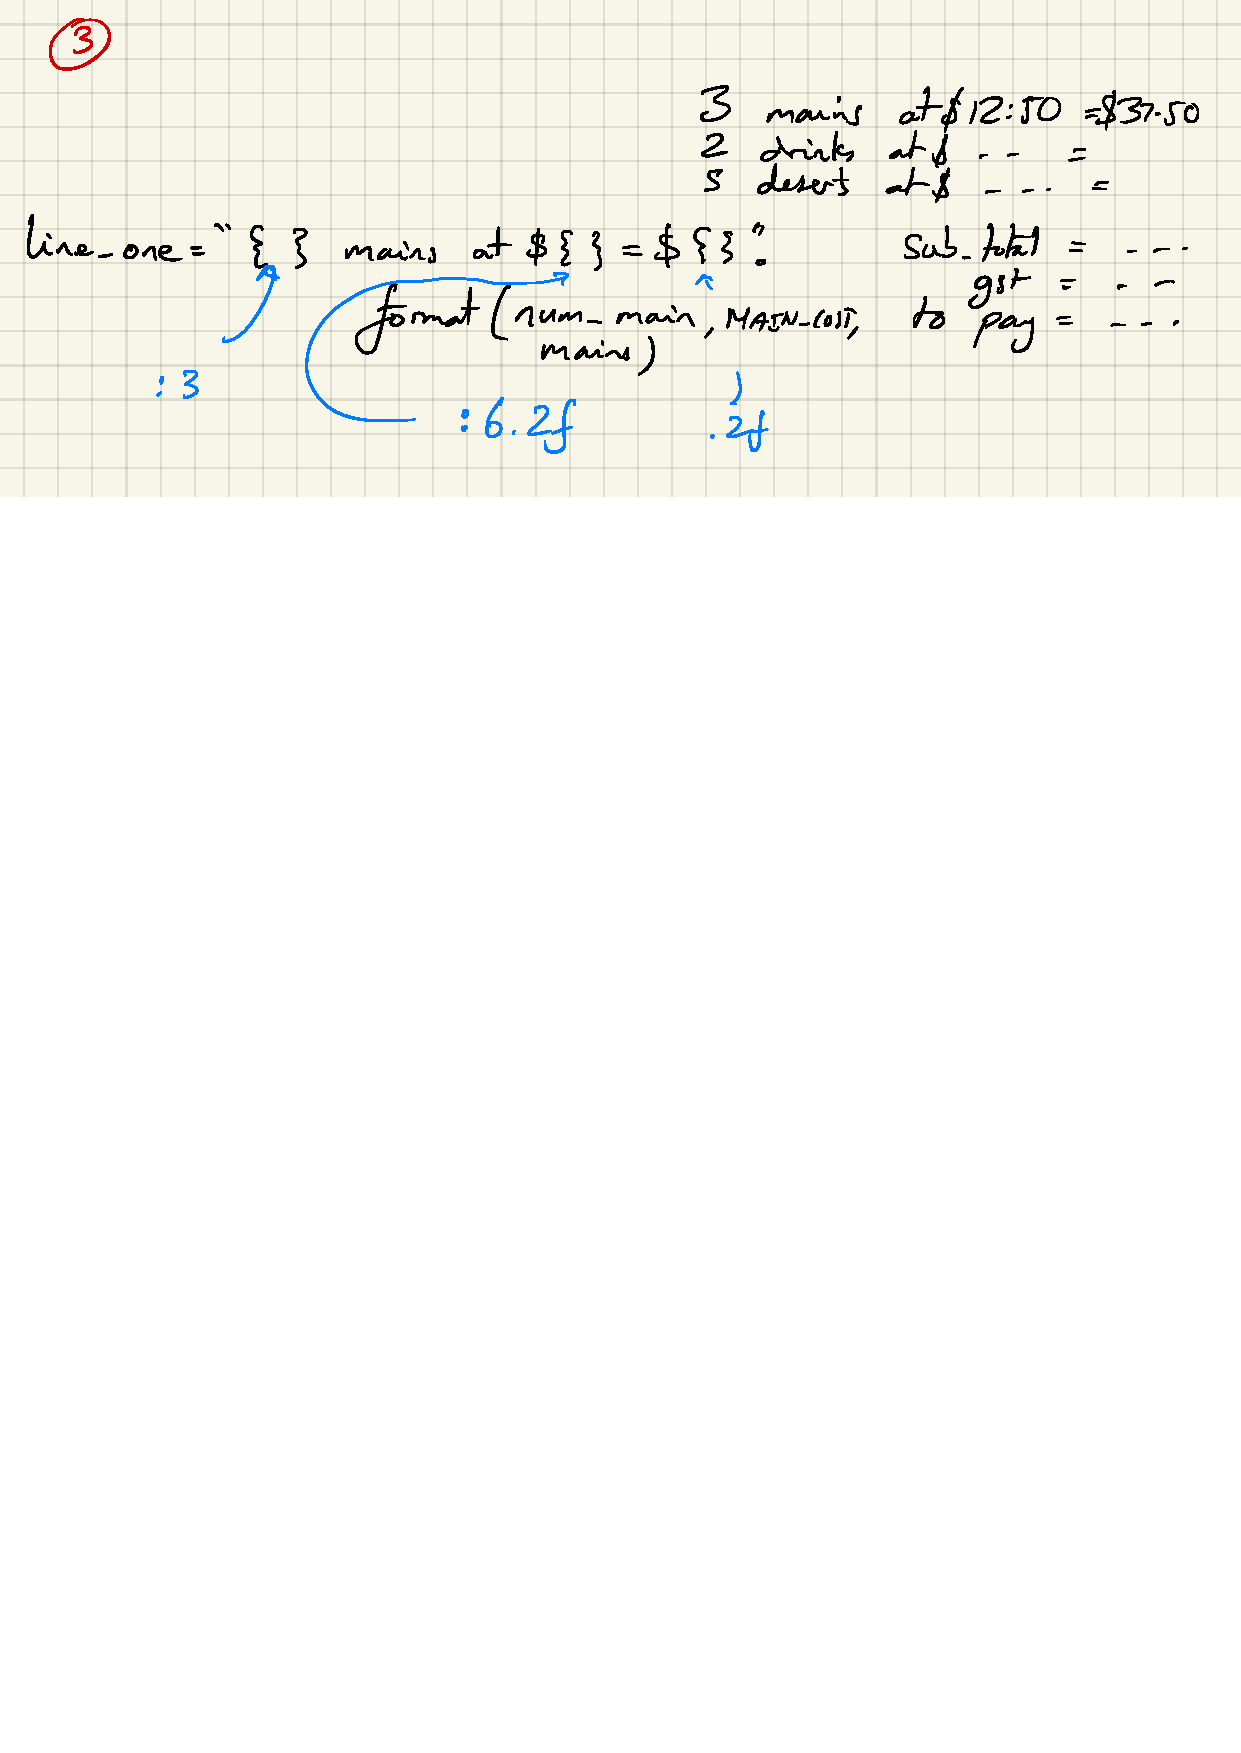
\includegraphics[width=12cm]{iterative_processes/simple_planning_2.pdf}
\end{figure}
\textbf{Basic Idea of Testing}
When testing we consider
\begin{itemize}
	\item Expected inputs (these are inputs we would normally expect the user to input).\\
	Does the porgram give the right outputs with the given expected inputs.
	\item Boundary inputs (are there maximum or minimum value that the user can enter)\\
	What happens at these \underline{boundaries} (and if we go over them)
	\item Unexpected Inputs  (these are character entries that we are not expecting)\\
	These could be just pressing enter or having spaces , using letters instead of numbers or characters like * , \&, etc.\\
	These could occur if the user makes a mistake or misunderstands what is expected.
\end{itemize}
Testing should have some kind of plan and documentation of the results.\\

\begin{figure} [!h]
	\centering
	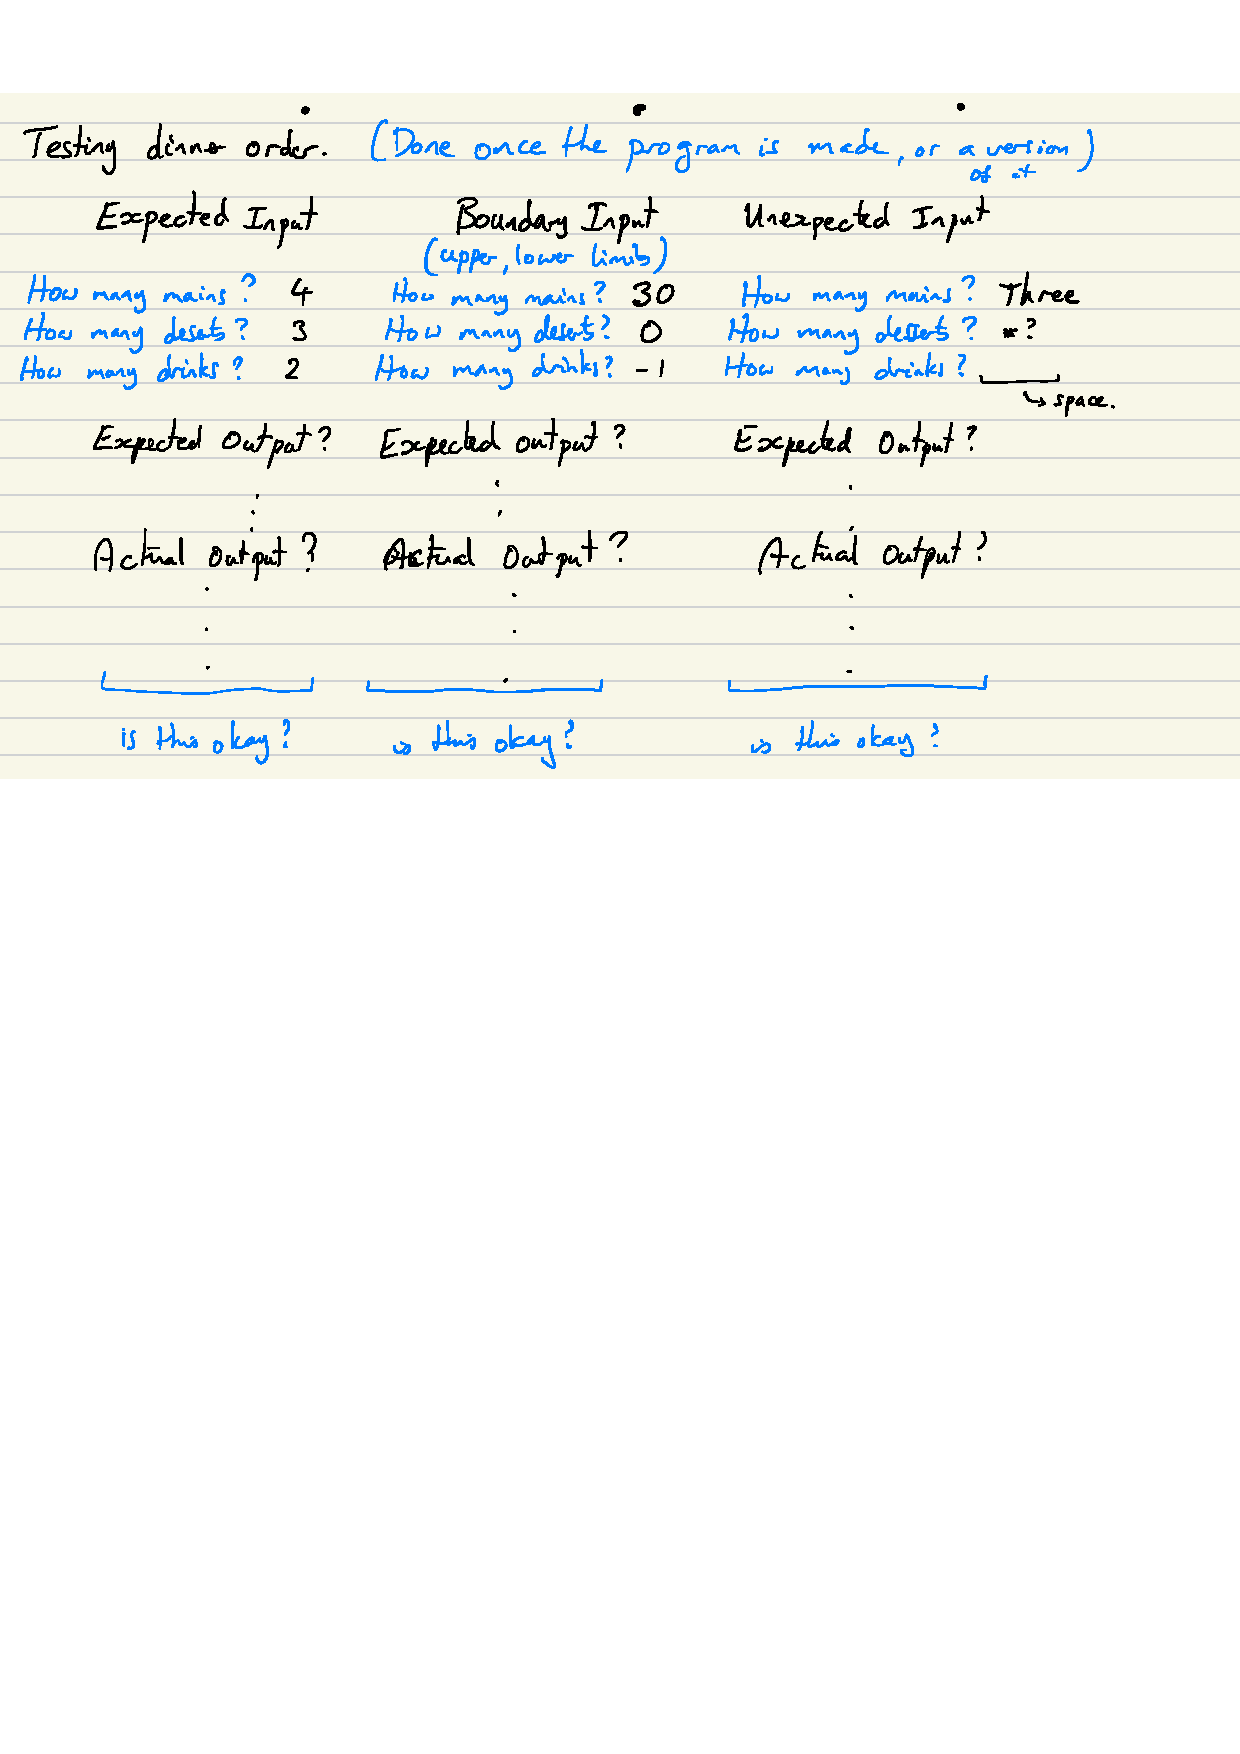
\includegraphics[width=16cm]{iterative_processes/Testing.pdf}
\end{figure}

\begin{figure} [!h]
	\centering
	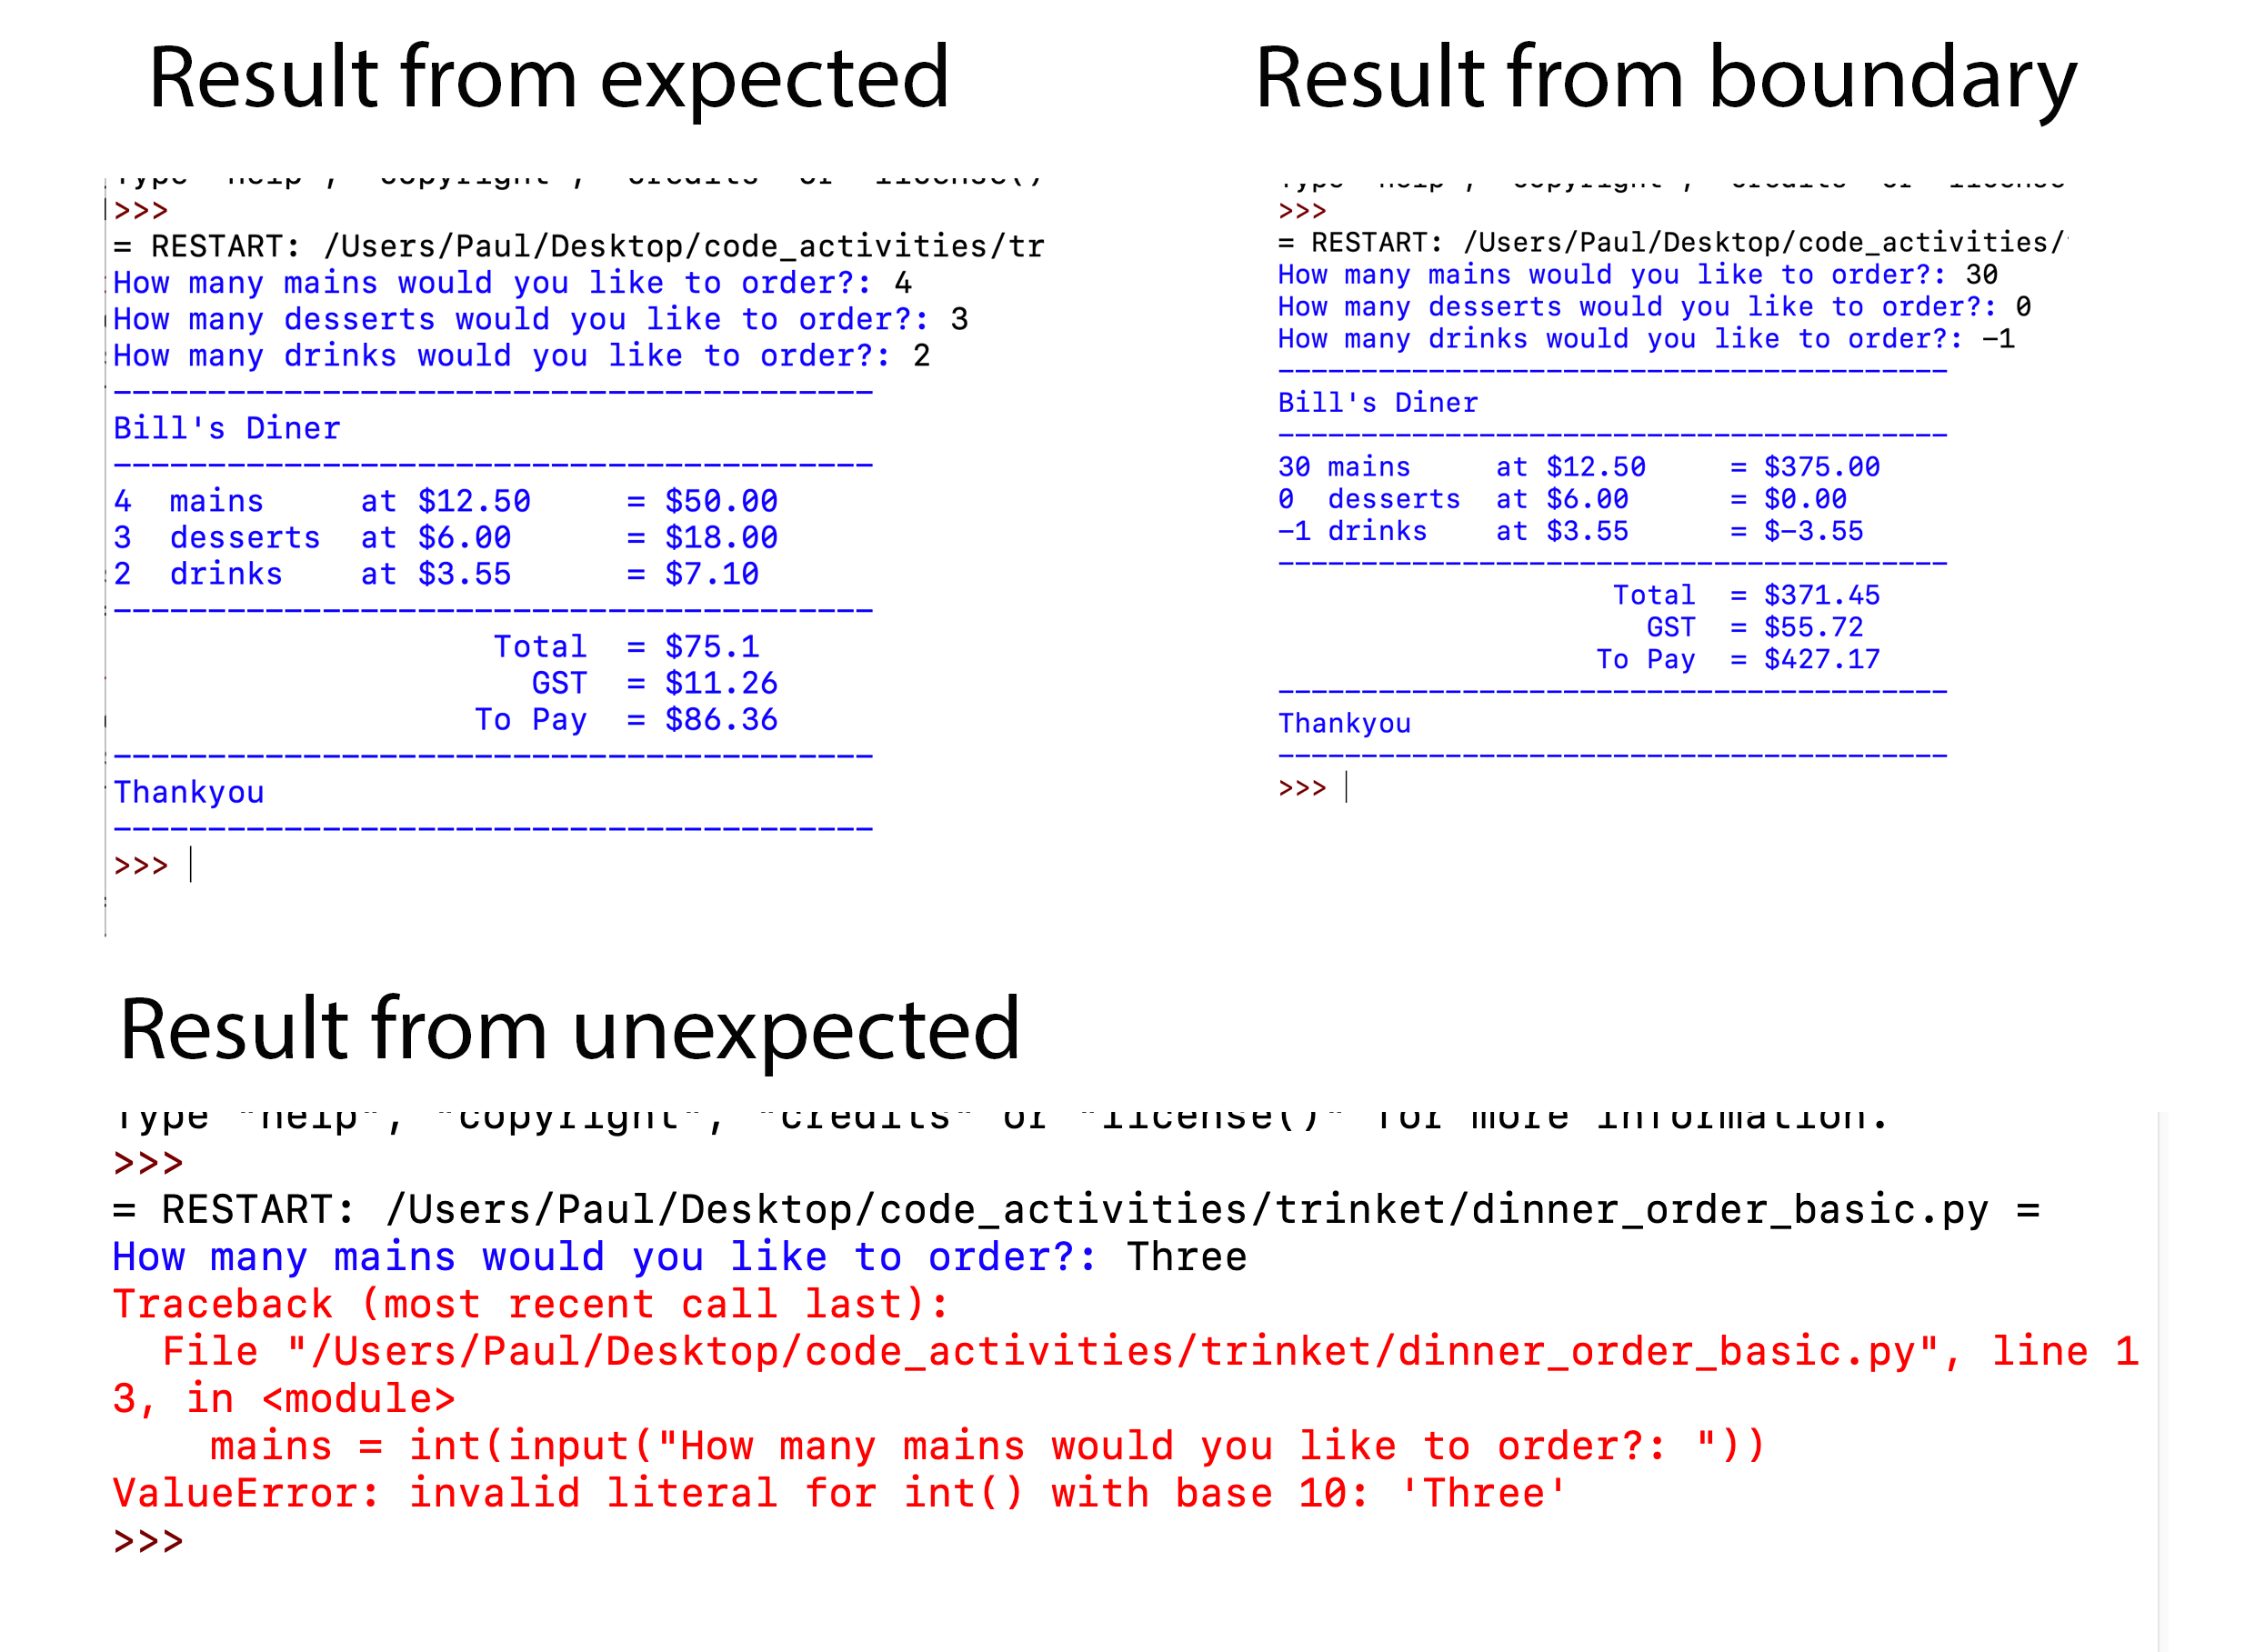
\includegraphics[width=16cm]{iterative_processes/Testing.png}
\end{figure}
\newpage
\textbf{Evaluation}
\begin{itemize}
	\item What works 
\begin{itemize}
	\item Works properly on expected inputs
	\item Presentation of reciept clearly laid out on console.
\end{itemize}
	\item What could be improved
\begin{itemize}
	\item Should have an upper limit on how many meals can be entered
	\item Should not allow entries below zero
	\item Unexpected inputs cause a program crash
	\item At the moment the program only runs once (so need a way to enter a new order)
\end{itemize}
\end{itemize}
\newpage
\begin{figure} [!h]
	\centering
	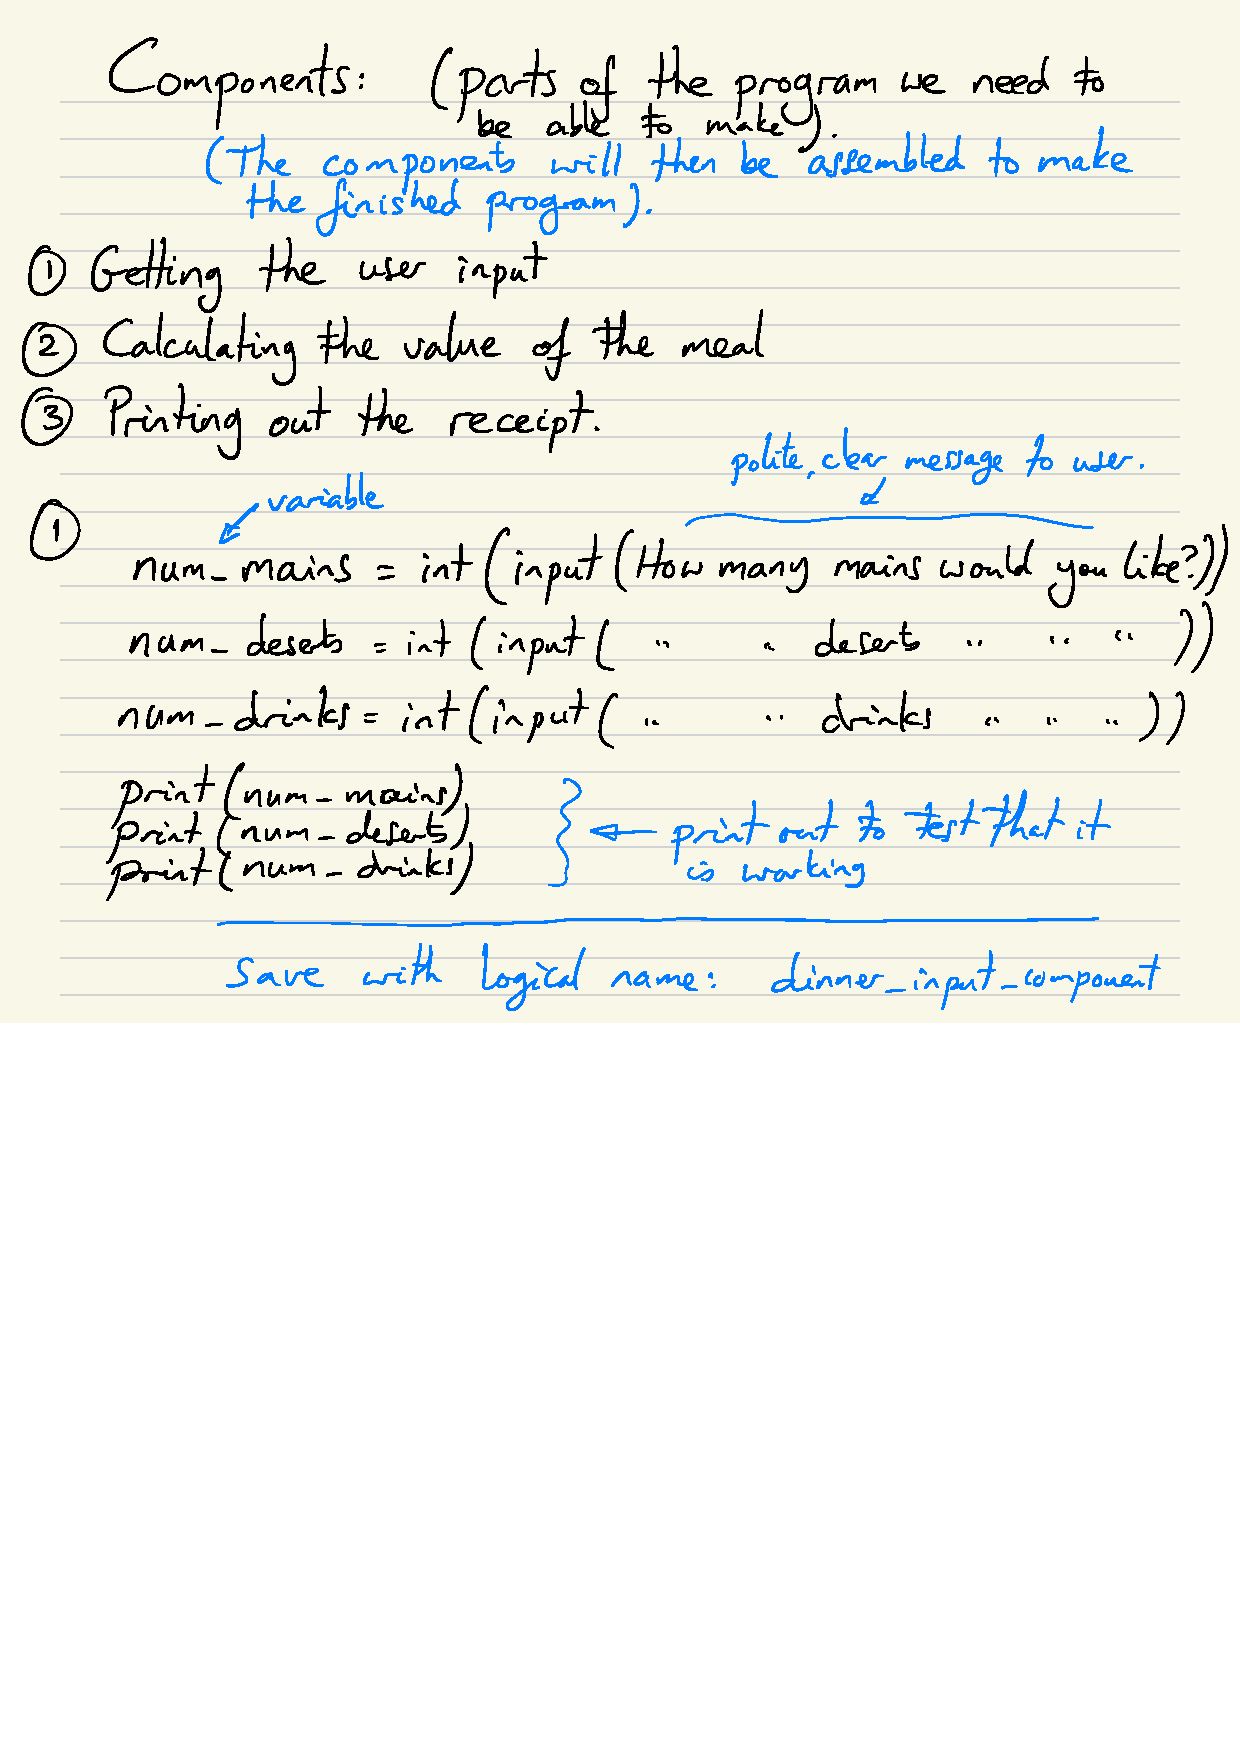
\includegraphics[width=12cm]{iterative_processes/Components_detailed_p1.pdf}
\end{figure}
\begin{figure} [!h]
	\centering
	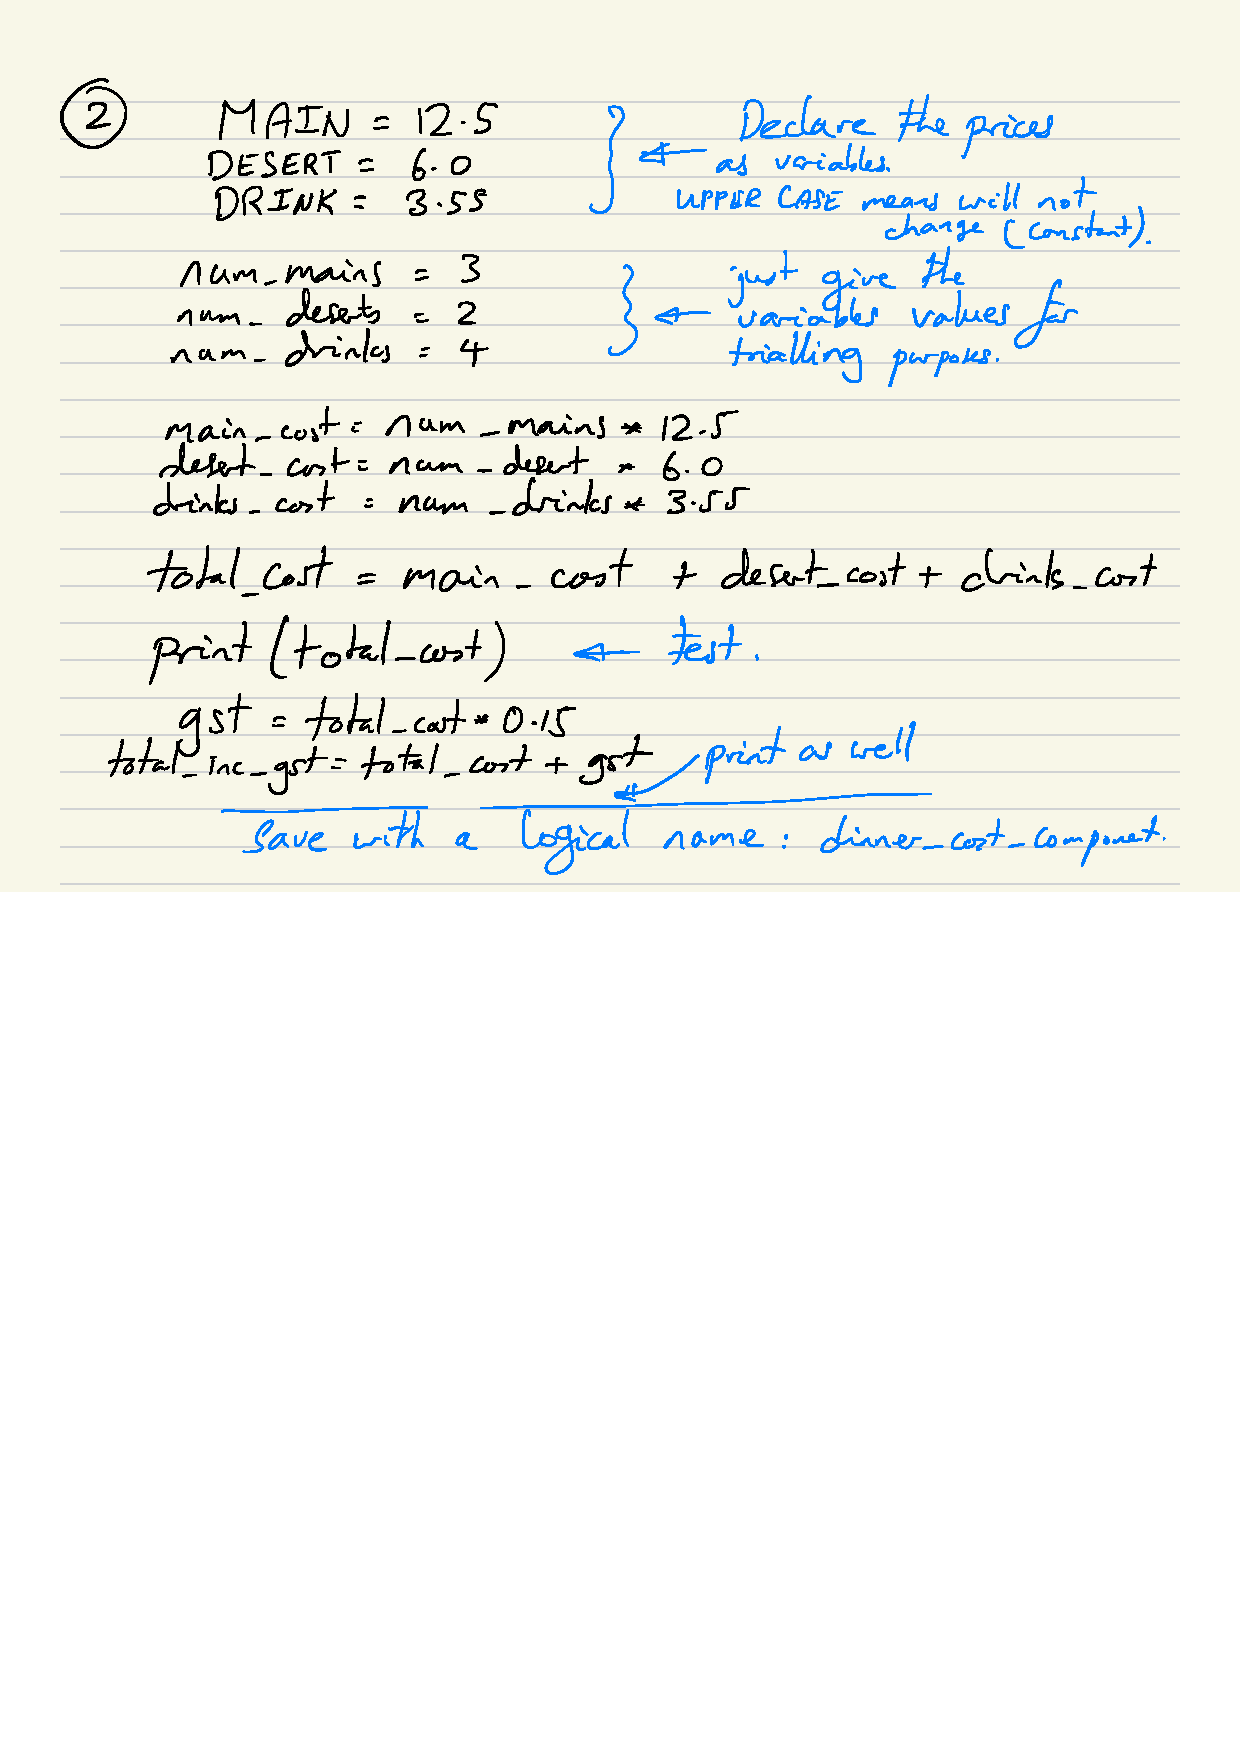
\includegraphics[width=12cm]{iterative_processes/Components_detailed_p2.pdf}
\end{figure}
\begin{figure} [!h]
	\centering
	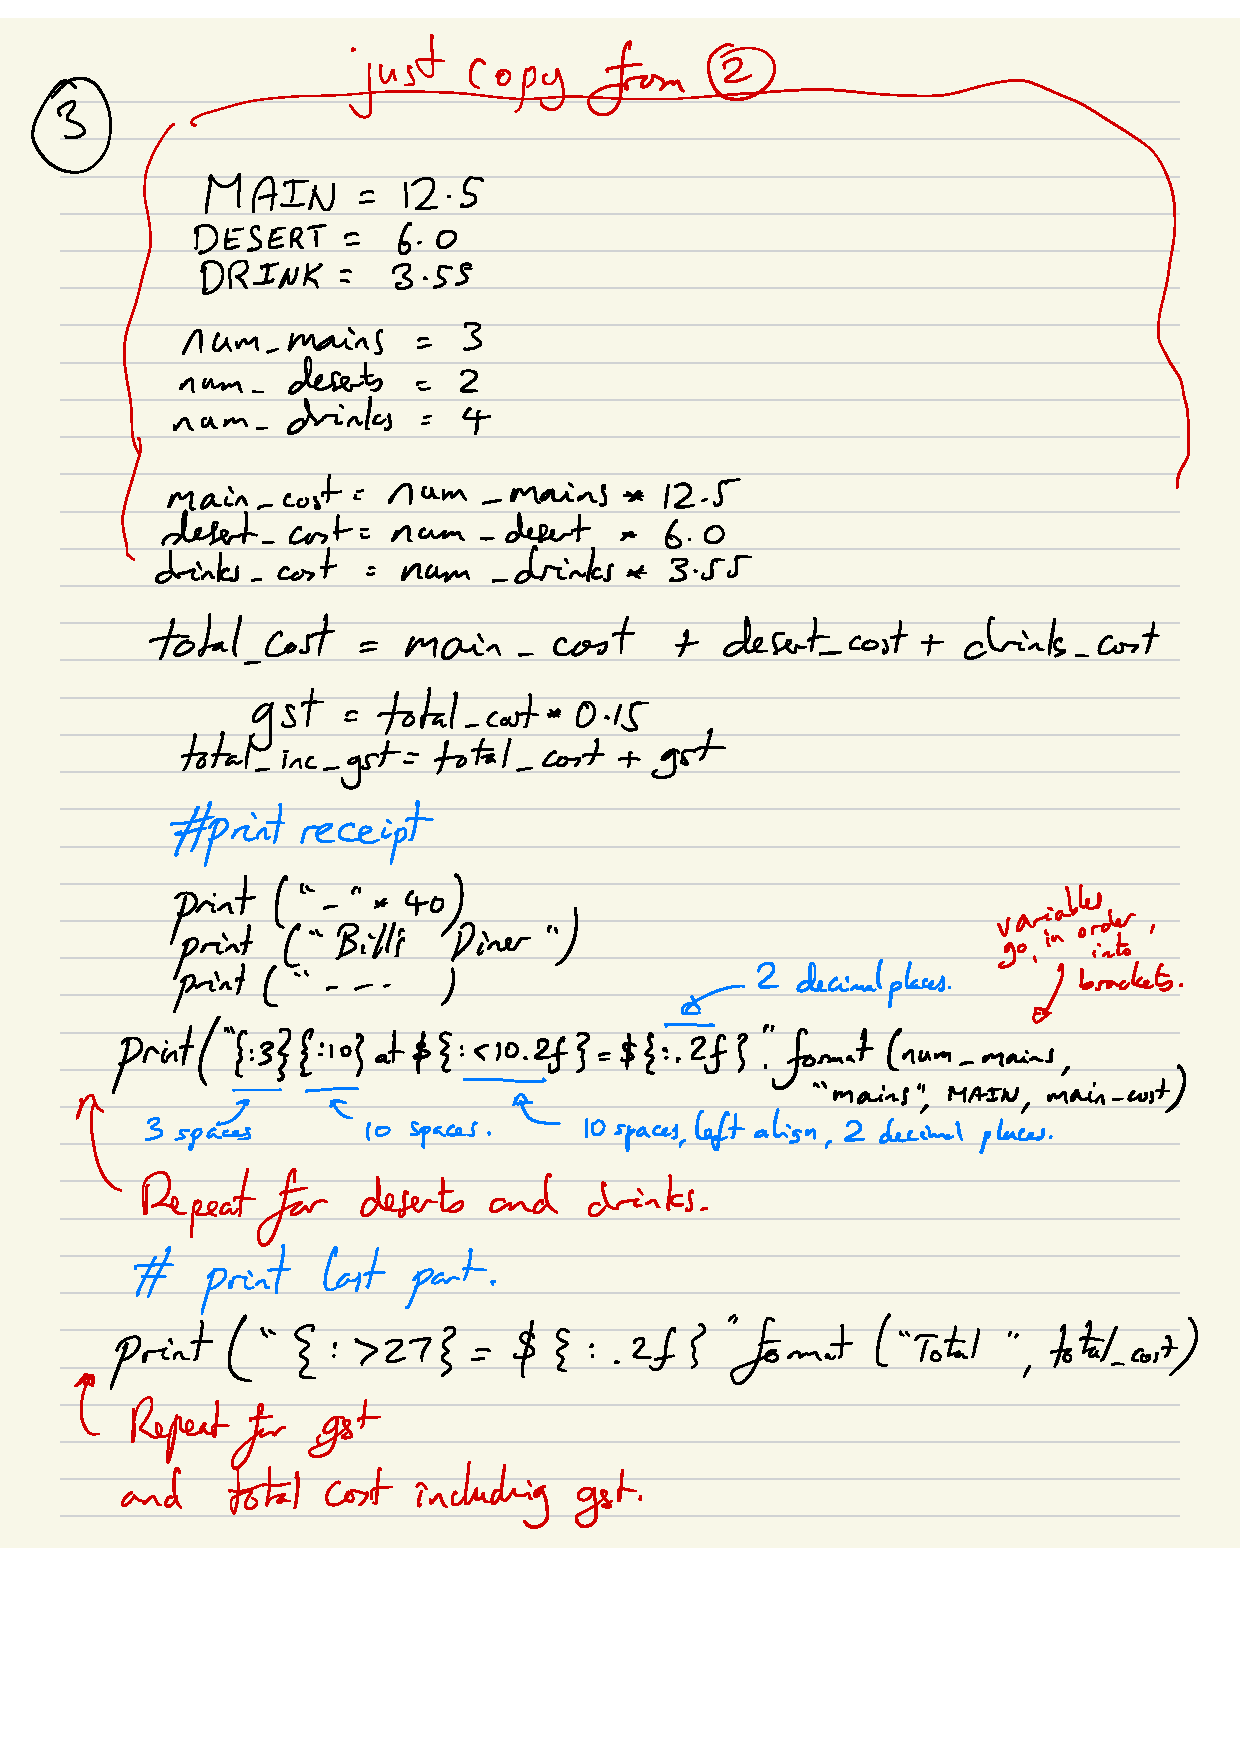
\includegraphics[width=12cm]{iterative_processes/Components_detailed_p3.pdf}
\end{figure}
\newpage


\lstinputlisting[language=Python, caption = Dinner Order Program]{trinket/dinner_order_basic.py}

\newpage

\lstinputlisting[language=Python, caption=Python example
]{strawberry_picking.py}

\newpage
\section{Conditions}
The solutions to many programming problems require an action to occur only if a particular condition is true.\\ 
A condition can only result in true or false. \\
(These values are called Booleans. True and False are reserved words in the Python language. True and False are values / objects of type bool)\\
A condition often involves an expression which compares one value with another.\\
Comparisons between numerical values are made using the same comparison operators that are used in mathematics:\\
\begin{align*}
> & \text{~~~~~~greater than}\\
>= & \text{~~~~~~greater than or equal to}\\
< & \text{~~~~~~less than}\\
<= & \text{~~~~~~less than or equal to}
\end{align*}
 and the equality / inequality operators:
 \begin{align*}
 ==  & \text{~~~~~~equal to ( the proper equals operator)}\\
 != & \text{~~~~~~not equal to}
 \end{align*}
\textbf{Boundary cases}\\
Human languages are imprecise. \\
Does "every child over 5" mean "aged 5 and over" or "aged 6 and over"? The difference between $>=$ and $>$ is very important. \\
If you mean "every child aged 5 and over" you can express this as age $> 4$ or age $>= 5$.\\
Any lack of clarity needs to be removed at the design phase. Always clarify before
coding. The boundary cases are where errors in programming often occur.\\
 Boundary cases are the values at and just outside the specified limits.\\
 In the case "aged 5 and over" the specified limit is 5 and the age values of 4 and 5 are the boundary cases.
 \newpage
 \begin{figure} [!h]
 	\centering
 	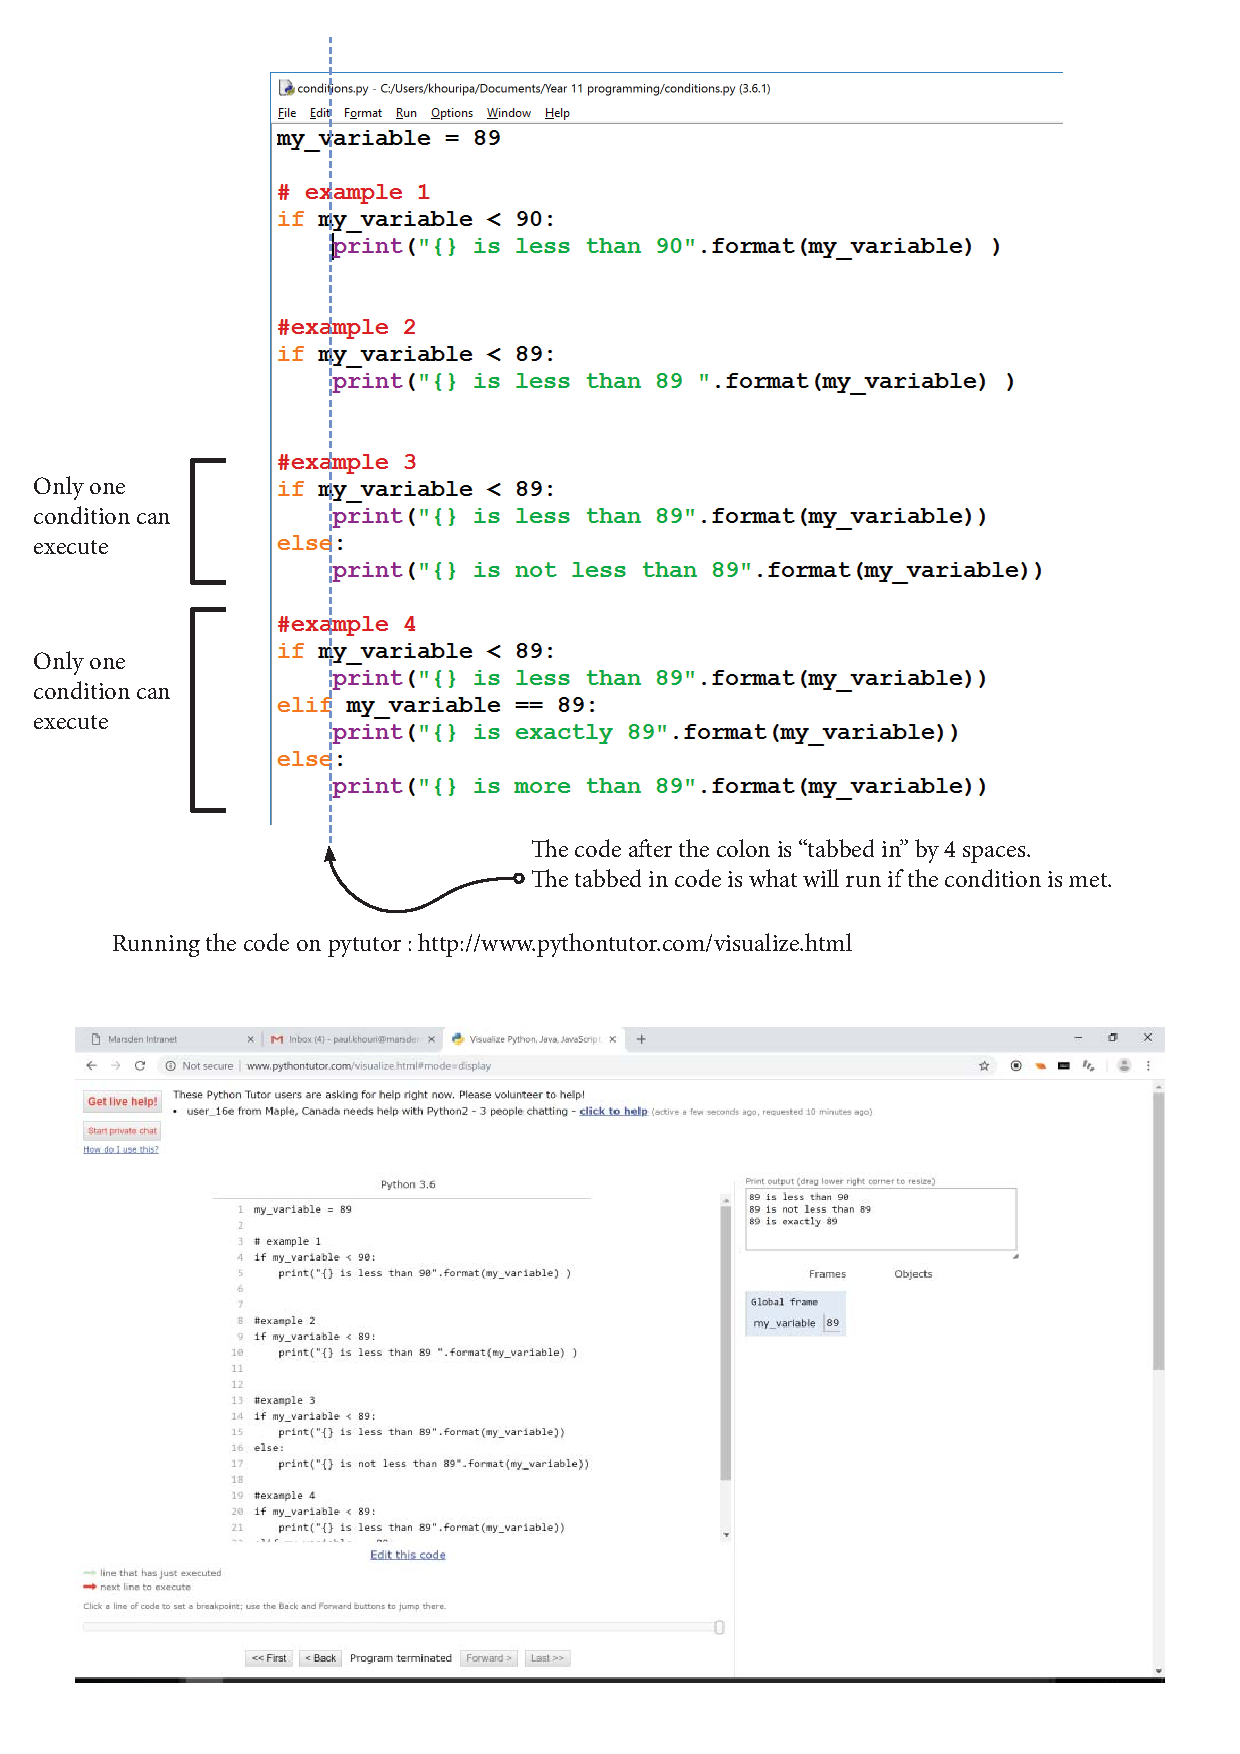
\includegraphics[width=17cm]{screen_shots/conditions.pdf}
 \end{figure}
\subsection{Activities}
\begin{enumerate}
	\item Consider a program that asks for a user’s age and then:
\begin{itemize}
	\item if their age 12 or less, tells them that they should be at primary school,
	\item if there age is more than 12 but less than 18, they need to go to secondary school
	\item if they are 18 years old, it tells them that they have become an adult
	\item and if they are older than 18 tells them that they must have left school.
\end{itemize}
\item 	To go to university a person needs to be:
\begin{itemize}
	\item over the age of 20
	\item \textbf{or} be 16 or older and have level 3 NCEA 
	\item \textbf{and} (for both conditions) the person need to be competent with English.
\end{itemize} 
Create a program that given the following variables:\\
age= 25\\
ncea = False\\
english = True\\
Will give a correct response about whether a person can go to university or not.\\
Test with other values.
\end{enumerate}

\newpage
\section{Random numbers}
\lstinputlisting[language=Python, caption=Python example]{randomness.py}
\section{Program using conditions and random numbers}
%\lstset{style=mystyle_big}
\lstinputlisting[language=Python, caption=Python example]{trinket/random_choose_L_E_H.py}
%\lstset{style=mystyle}
\newpage
\section{Loops}
\section{Lists}
\section{Functions}
\lstinputlisting[language=Python, caption=Python example]{addition_question.py}
\lstinputlisting[language=Python, caption=Python example]{function_tests.py}

\section{Dictionaries}
\lstinputlisting[language=Python, caption=Python example]{dictionaries.py}
\lstinputlisting[language=Python, caption=Python example]{tommi.py}
\section{Validation}
\lstinputlisting[language=Python, caption=Python example]{validation_example.py}


\newpage
\section{Coffee}
\lstinputlisting[language=Python, caption=Python example]{class_randomletters_function.py}
\lstinputlisting[language=Python, caption=Python example]{buildingastring.py}
\lstinputlisting[language=Python, caption=Python example]{buildingastring_v2.py}
\lstinputlisting[language=Python, caption=Python example]{buildingastring_v3.py}
\lstinputlisting[language=Python, caption=Python example]{class_randomletters_testfor6.py}
\lstinputlisting[language=Python, caption=Python example]{class_randomletters_function_c_list.py}
\lstinputlisting[language=Python, caption=Python example]{class_randomletters_function_list.py}
\lstinputlisting[language=Python, caption=Python example]{class_randomletters_testfor7.py}
\lstinputlisting[language=Python, caption=Python example]{class_randomletters_testfor8.py}
\lstinputlisting[language=Python, caption=Python example]{class_randomletters.py}
\lstinputlisting[language=Python, caption=Python example]{class_randomletters_function_c.py}
\lstinputlisting[language=Python, caption=Python example]{class_randomletters_to_distribution.py}
\newpage
\section{Tests}
\lstinputlisting[language=Python, caption=Dice Roll]{v0_random.py}
\lstinputlisting[language=Python, caption=Python example]{checkinlist.py}
\lstinputlisting[language=Python, caption=Python example]{dictionary_test.py}
\lstinputlisting[language=Python, caption=Python example]{format_test.py}
\lstinputlisting[language=Python, caption=Python example]{hangman.py}
\section{Strings}
\lstinputlisting[language=Python, caption=Python example]{string_tests.py}
\lstinputlisting[language=Python, caption=Python example]{counting_string.py}
\section{Objects}
\lstinputlisting[language=Python, caption=Python example
]{classes_objects.py}

\lstinputlisting[language=Python, caption=Python example
]{classforglobals.py}

\lstinputlisting[language=Python, caption=Python example
]{class_quiz.py}













\end{document}